\section{分子動力学(MD)シミュレーション}

分子動力学シミュレーションにより、$\beta_2$ARのinactive状態active状態双方で1000psトラジェクトリを計10本取得した。

\subsubsection{$\beta_2$ARの活性化による構造変化}
アゴニストが結合した$\beta_2$ARは、顕著な構造変化を引き起こす\cite{rasmussen2011crystal}ことがわかっている。
%参考文献:β2ARの構造変化
%2011「β2アドレナリン受容体-Gsタンパク質複合体の結晶構造」
%https://www.nature.com/articles/nature10361
主な変化として以下が挙げられる:
\begin{enumerate}
    \item \textbf{TM6の移動}: TM6の細胞質側末端が、約14Å外側に移動する。この移動により、Gタンパク質が結合するための空間が確保される。
    \item \textbf{TM5の変化}: TM5の細胞質側末端部分において、αヘリックスが2回転分引き伸ばされる。これにより、シグナル伝達に関与する構造が再編成される。
\end{enumerate}

本研究で得られた、シミュレーション中の原子の平均的な配置を示した$\beta_2$ARのinactive構造とactive構造を重ね合わせたのが以下の図である。
%inactiveとactiveの重ね合わせ
\begin{figure}[htbp]
  \centering
  \begin{subfigure}{0.45\textwidth} % 各図の幅を調整
    \centering
    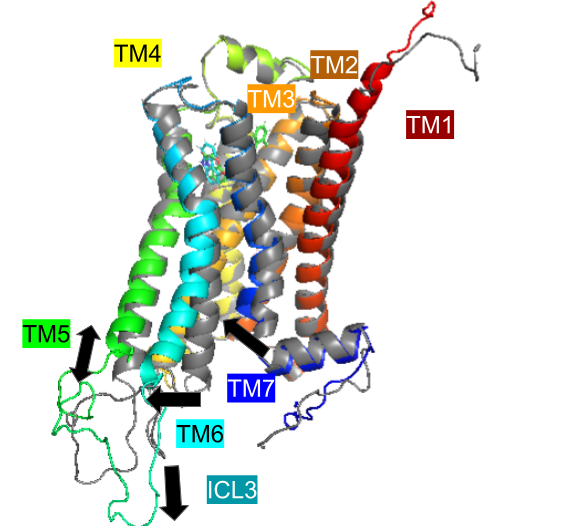
\includegraphics[width=\textwidth]{system-all-with-label.png}
    \caption{$\beta_2$ARのTM5,TM6,TM7の変化。}
    \label{fig:fitting_TM}
  \end{subfigure}
  \hspace{0.05\textwidth} % 図の間のスペース
  \begin{subfigure}{0.45\textwidth}
    \centering
    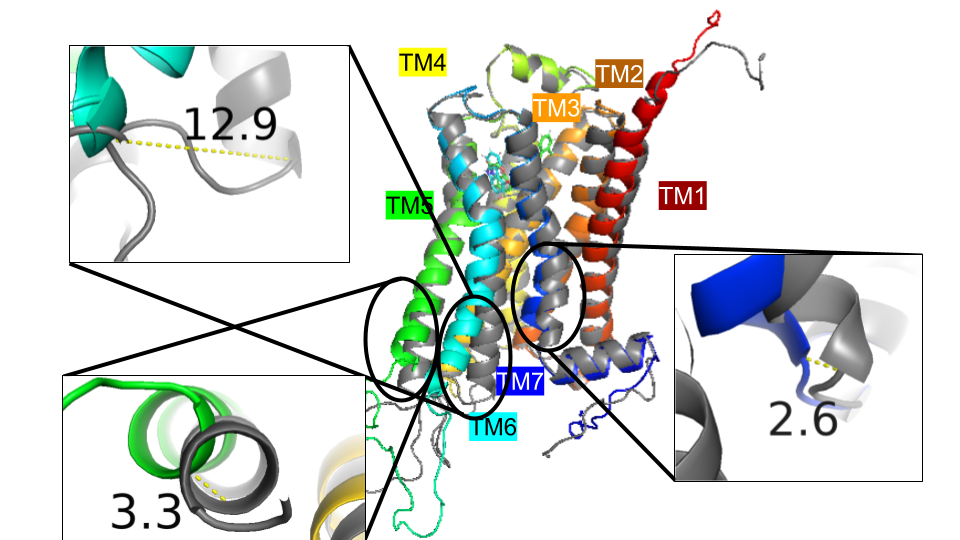
\includegraphics[width=\textwidth]{system-all-with-label-detail.png}
    \caption{$\beta_2$ARのTM5,TM6,TM7の変化の詳細。}
    \label{fig:fitting_TM_detail}
  \end{subfigure}
  \caption{$\beta_2$ARのinactive構造(グレー)とactive構造(色付き)の重ね合わせ。}
  \label{fig:fitting-all}
\end{figure}

TM6の細胞質側末端にある残基のCα原子が、TM7から離れる方向に12.9Å移動する様子が観察された。
TM5の細胞質側末端部分は2残基分の延長が観察されるとともに、末端のCα原子がTM6から離れる方向に3.3Å移動する様子が観察された。
また、TM7の細胞質側末端にある残基のCα原子が、タンパク質の内側に近づく方向に2.6Å移動する様子が観察された。

\subsubsection{$\beta_2$ARの保存された結晶水}
DOWSERによって検出された、エネルギー的に安定な水分子は、inactive状態で14869個、active状態で18876個同定された。
そのうち、シミュレーション中で保存されている結晶水はinactive状態で7個、active状態で5個同定された。

\begin{figure}[htbp]
    \centering
    \begin{subfigure}{0.45\textwidth} % 各図の幅を調整
      \centering
      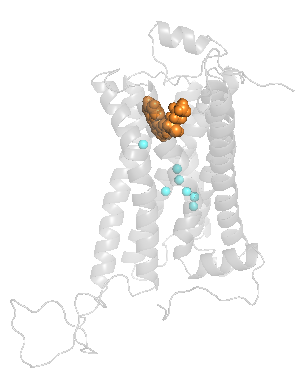
\includegraphics[width=\textwidth]{inactive_saved_water.png}
      \caption{$\beta_2$ARのinactive状態における保存された結晶水。}
      \label{fig:inactive_water}
    \end{subfigure}
    \hspace{0.05\textwidth} % 図の間のスペース
    \begin{subfigure}{0.45\textwidth}
      \centering
      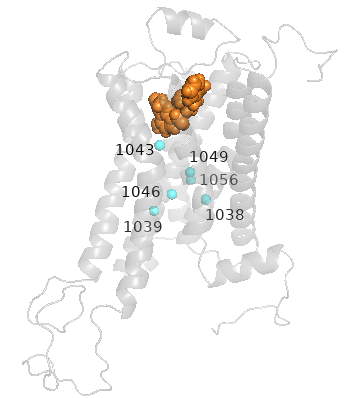
\includegraphics[width=\textwidth]{active_saved_water.png}
      \caption{$\beta_2$ARのactive状態における保存された結晶水。}
      \label{fig:active_water}
    \end{subfigure}
    \caption{保存された結晶水}
    \label{fig:water-all}
  \end{figure}

\newpage

%inactiveとactiveで保存されている結晶水


%先行研究との比較

\section{$\beta_2$ARのinactiveおよびactive状態のコミュニティ検出}

得られた座標データを基に、ネットワークのエッジの重みとして用いる残基間最短距離の2乗逆数の平均\langle \frac{1}{d^2} \rangle を計算した。

エッジを以下の条件で形成させた後、エッジの重みを加え、inactive状態active状態双方のネットワークを構築した。
1. 残基ペア間の最短距離が3\,\text{\AA}未満である場合、エッジを形成する。
2. アミノ酸配列上で隣接する残基感のエッジは削除する。

以下が構築されたネットワークの詳細である。
\begin{table}[!ht]
    \centering
    \caption{ネットワーク上のノード数と、残基ペア間の最短距離が3\,\text{\AA}未満のエッジ数}
    \begin{tabular}{lll}
      \hline
      モデル名          & ノード数  & エッジ数 \\
      \hline 
      inactive(3P0G)  &  351 &  16336 \\ 
      active(2RH1)    &  349 &  15433 \\ 
    \end{tabular}
    \label{tab:network_size}
  \end{table}

構築されたネットワークを基に、コミュニティ検出を行った。
\subsubsection{Louvain法の信頼性}

ネットワークにおけるコミュニティ構造を検出するために用いたLouvain法の結果の信頼性は、モジュラリティ$Q$の値を用いて評価される。
モジュラリティ$Q$の値は通常-1から1の範囲を取り、以下のように解釈される:

\begin{itemize}
    \item \( Q \) が負:分割がネットワーク構造と一致しておらず、不適切な分割である。
    \item \( Q \) が 0 に近い:ネットワークがランダム構造に近い。
    \item \( Q \) が正:ネットワーク内にコミュニティ構造が存在する。
\end{itemize}

本研究の解析対象である$\beta_2$ARのinactiveおよびactive状態のコミュニティ検出におけるモジュラリティ$Q$の最良値および標準偏差を計算した。

\paragraph{試行回数100回におけるモジュラリティ値の平均および標準偏差}
\begin{itemize}
    \item inactive状態: \( Q = 0.5172 \pm 0.0059 \)
    \item active状態: \( Q = 0.5239 \pm 0.0044 \)
\end{itemize}
さらに、モジュラリティ値の標準誤差は以下の通りです:
\begin{itemize}
    \item inactive状態: \( \pm 0.0006 \)
    \item active状態: \( \pm 0.0004 \)
\end{itemize}

inactive状態とactive状態のモジュラリティ値はどちらも正の値を示しており、ネットワーク内に明確に分割されたコミュニティ構造があることを示唆している。

\subsection{Louvain法で検出されたコミュニティ}

以下に$\beta_2$ARのinactive構造とactive構造で検出されたコミュニティを示す。

\begin{figure}[htbp]
    \centering
    \begin{subfigure}{0.45\textwidth} % 各図の幅を調整
      \centering
      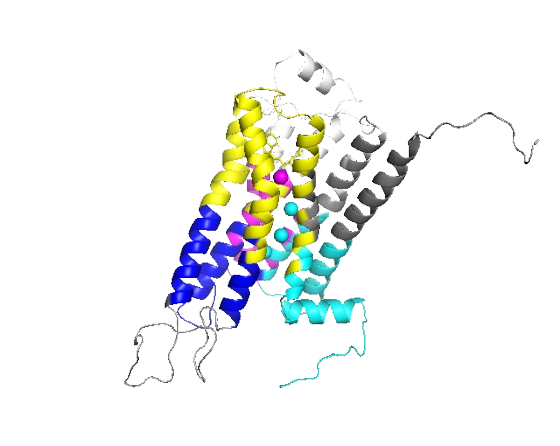
\includegraphics[width=\textwidth]{inactive.png}
      \caption{$\beta_2$ARのinactive状態において検出されたコミュニティ構造を色分けして示した図。各色と名付けたコミュニティは以下に表す:黒(start)、シアン(end)、白(helix)、ピンク(back)、グレー(loop)、黄色(ligand)、青(gprotein)。}
      \label{fig:inactive_community}
    \end{subfigure}
    \hspace{0.05\textwidth} % 図の間のスペース
    \begin{subfigure}{0.45\textwidth}
      \centering
      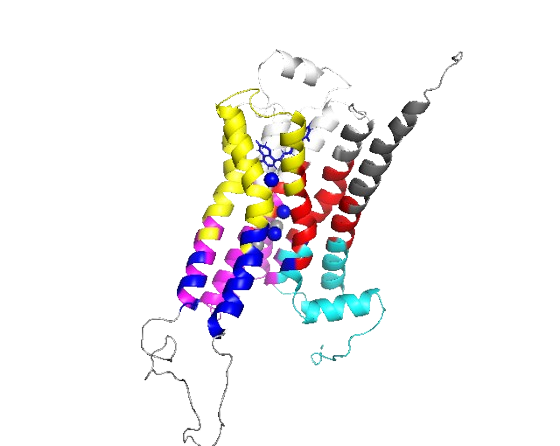
\includegraphics[width=\textwidth]{active.png}
      \caption{$\beta_2$ARのactive状態において検出されたコミュニティ構造を色分けして示した図。各色と名付けたコミュニティは以下に表す:黒(start)、シアン(end)、白(helix)、ピンク(back)、グレー(loop)、黄色(ligand)、青(gprotein)、赤(new)。}
      \label{fig:active_community}
    \end{subfigure}
    \caption{コミュニティ構造}
    \label{fig:community-all}
  \end{figure}

\newpage

まず双方のコミュニティに共通することとして、リガンド結合部位と活性部位であるGタンパク質結合部位に対応する独立したコミュニティが、黄色(ligand)、青(gprotein)として検出された。
また図\ref{fig:inactive}から図\ref{fig:active}への変化として、青(gprotein)コミュニティの再編成が起きていることと、赤(new)コミュニティが新規に形成されたことが挙げられる。

青(gprotein)コミュニティと赤(new)コミュニティに属する残基の比較を行うと、以下のようになる。

%比較したtableを追加

active状態になると、青(gprotein)コミュニティにはリガンドと保存された結晶水3つ、赤(new)コミュニティにはモチーフが追加された。
%何のモチーフ

ここで、図\ref{fig:inactive}と図\ref{fig:active}で示されているネットワークの全体密度を計算する。
全体エッジ密度$D_{\text{global}}$の計算式は以下のように表される。

\[
W_{\text{actual}} = \sum_{(u, v) \in E} w(u, v)
\]

W_{\text{actual}}は実際のエッジ重みの合計である。
$E$は、グラフ内のエッジ集合を示す。
$w(u, v)$は、エッジ$(u, v)$の重みを示す。

\[
W_{\text{max}} = \sum_{i=1}^{N} \sum_{j=i+1}^{N} w(i, j)
\]

W_{\text{max}}は理論上可能な最大エッジ重みの合計である。
$N$は、グラフ内のノード数を示す。
$w(i, j)$は、ノード$i$と$j$の間のエッジ重みを示す。

\[
D_{\text{global}} = \frac{W_{\text{actual}}}{W_{\text{max}}}
\label{eq:global_density}
\]

最終的に、ネットワークの全体エッジ密度$D_{\text{global}}$は以上のように示される。

この式に基づいて、inactive構造とactive構造のネットワークの全体エッジ密度を計算すると、それぞれ以下のようになる。
\begin{itemize}
    \item inactive状態:\( Q = 0.3083 \)
    \item active状態:\( Q = :0.8579 \)
\end{itemize}

inactive状態は低い密度を示しており、最短距離が3\,\text{\AA}未満の残基ペアが相対的に少なかった。
active状態は、inactive状態に比べて高い全体エッジ密度を持っており、より多くの相互作用が存在することを示している。この結果は、活性状態におけるタンパク質の構造や機能がより密接に結びついていることを示唆している。

\subsection{コミュニティ内およびコミュニティ間のエッジ密度}
active状態で再編成されたコミュニティや新しく検出されたコミュニティの役割を定量的に分析するために、ネットワークの全体密度$D_{\text{global}}$の計算で用いた密度の概念を用いたさらなる計算を行った。
続いて、inactive状態とactive状態双方においてそれぞれコミュニティ内のエッジ密度、コミュニティ間のエッジ密度を計算した。

\subsubsection{コミュニティ内エッジ密度}
コミュニティ内エッジ密度$D_{\text{internal}}$の計算式は以下のように表される。

まずコミュニティごとにサブグラフを作成する。
ただしコミュニティ間のエッジは削除し、独立したコミュニティを表現している。
続いてコミュニティ内エッジ密度を計算する。

\[
D_{\text{internal}} = \frac{\sum_{(u,v) \in E_C} w_{uv}}{\sum_{(u,v) \in E_C} w_{uv}^{\text{max}}}
\label{eq:internal_density}
\]

ここで$E_C$はコミュニティ$C$内の全エッジの集合、$w_{uv}$はノード$u$とノード$v$の間の実際のエッジ重み、$w_{uv}^{\text{max}}$はノード$u$とノード$v$の間のエッジの最大可能重みである。

分子の\(\sum_{(u,v) \in E_C} w_{uv}\)はコミュニティに属するノード間に存在する実際のエッジの重みの合計を示している。
分母の \(\sum_{(u,v) \in E_C} w_{uv}^{\text{max}}\) は、
そのコミュニティ内の全てのノードが完全に接続している場合のエッジの最大可能重みの合計を示している。

ただし、自己ループは除く。


コミュニティ内エッジ密度$D_{\text{internal}}$は、ネットワーク全体のエッジ密度を基準としてコミュニティ内のエッジ密度がネットワーク全体と比べて相対的にどれだけ高い(または低い)かを示し、コミュニティ内部でどれだけ密接に関連しているかを測定することを目的としている。
上記の式に基づいて、inactive構造とactive構造のコミュニティ内エッジ密度を計算すると、それぞれ以下のようになる。

\begin{figure}[htbp]
    \centering
    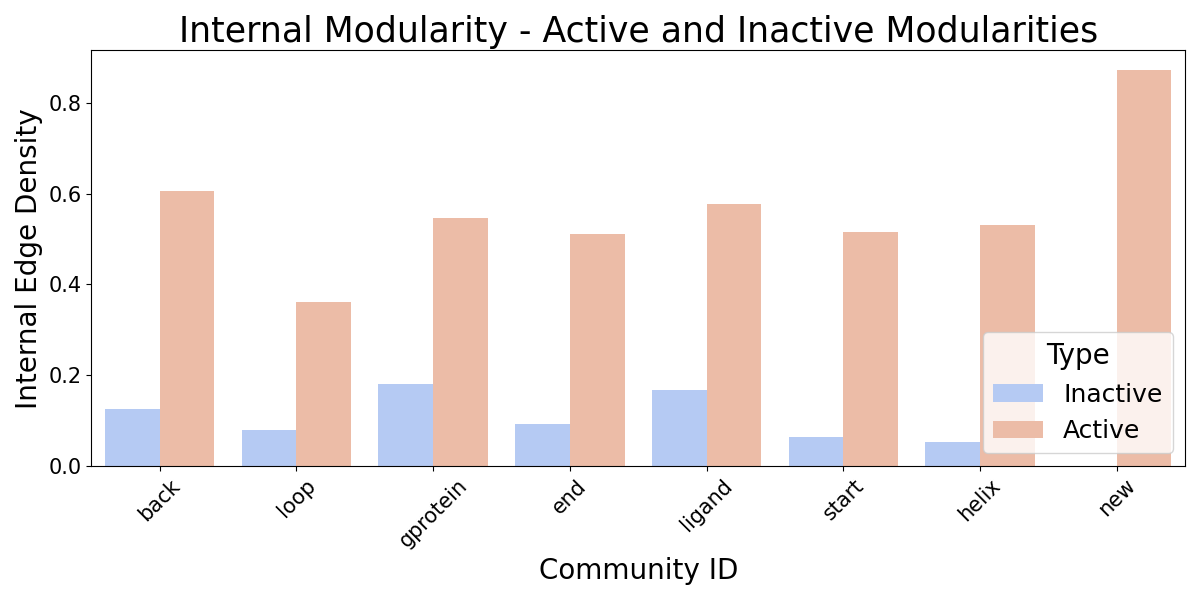
\includegraphics[width=0.8\textwidth]{internal_modularities.png}
    \caption{$\beta_2$ARのinactive状態とactive状態において検出されたコミュニティのコミュニティ内エッジ密度を示した図。コミュニティの名称は、図\ref{fig:inactive}と図\ref{fig:active}で名付けたものである。}
    \label{fig:internal}
\end{figure}

\newpage

コミュニティ内エッジ密度$D_{\text{internal}}$の値は以下のように解釈される:
\begin{itemize}
    \item \( D_{\text{internal}} \) が 0 に近い:コミュニティ内のノード間の相互作用は希薄であり、結びつきが弱い。
    \item \( D_{\text{internal}} \) が 1 に近い:コミュニティ内のノード間には強い結びつきがあり、密に相互作用している。
\end{itemize}

inactive構造では、loop, newコミュニティのコミュニティ内エッジ密度が特に大きい値を示した。
一方でactive構造においては、全てのコミュニティのコミュニティ内エッジ密度が1.0付近という値を示し、特に強い結びつきを形成している構造であることがわかる。
inactive構造からactive構造への変化に着目すると、どのコミュニティも値が大幅に大きくなり、特にgproteinコミュニティが顕著であった。

\subsubsection{コミュニティ間エッジ密度}
コミュニティ間エッジ密度$D_{\text{inter}}$の計算式は以下のように表される。

\[
D_{\text{inter}} = \frac{\sum_{\substack{u \in C_i \\ v \in C_j}} w_{uv}}{\sum_{\substack{u \in C_i \\ v \in C_j}} w_{uv}^{max}}
\label{eq:inter_density}
\]

ここで$C_i$と$C_j$はそれぞれ異なるコミュニティ$i$と$j$、$w_{uv}$はノード$u$とノード$v$の間の実際のエッジ重み、$w_{uv}^{\text{max}}$はノード$u$とノード$v$の間のエッジの最大可能重みである。
分子の \sum_{\substack{u \in C_i \\ v \in C_j}} w_{uv} は異なるコミュニティに属するノード間の実際のエッジの重みの合計を示している。
分母の \sum_{\substack{u \in C_i \\ v \in C_j}} w_{uv}^{max} は、そのコミュニティ間の全てのノードが完全に接続している場合のエッジの最大可能重みの合計を示している。
ただし、自己ループは除く。

コミュニティ間エッジ密度は、異なるコミュニティ間のエッジの結びつきの強さを示しており、お互いにどれだけ相互作用が強いかを測定することを目的としている。
上記の式に基づいて、inactive構造とactive構造のコミュニティ間エッジ密度を計算すると、それぞれ以下のようになる。

\begin{figure}[htbp]
    \centering
    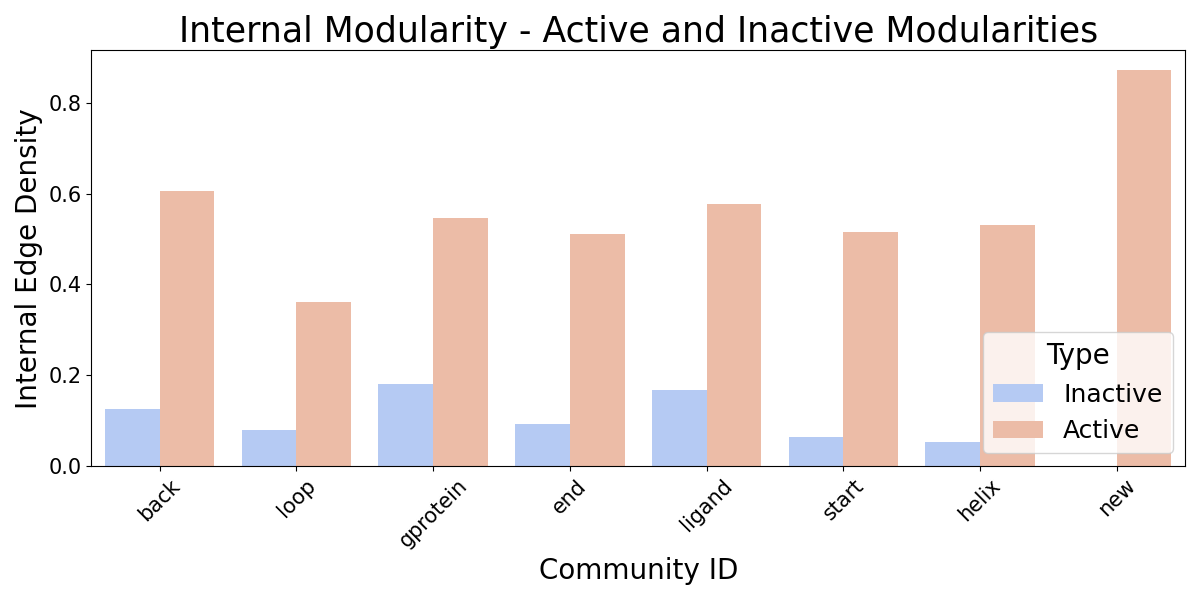
\includegraphics[width=0.8\textwidth]{internal_modularities.png}
    \caption{$\beta_2$ARのinactive状態とactive状態において検出されたコミュニティのコミュニティ間エッジ密度を示した図。コミュニティの名称は、図\ref{fig:inactive}と図\ref{fig:active}で名付けたものである。}
    \label{fig:inter}
\end{figure}

\newpage

ただし、inactive状態とactive状態の双方でコミュニティ間エッジ密度が0だったコミュニティペアは、図から除外している。
該当するコミュニティペアはstart-loop、helix-loop、new-loopである。

コミュニティ間エッジ密度$Q$の値は以下のように解釈される:
\begin{itemize}
    \item \( Q \) が 0 に近い:コミュニティ間でエッジが少なく、各コミュニティがほぼ独立している。
    \item \( Q \) が 1 に近い:コミュニティ間で多数のエッジが存在し、コミュニティ間の結びつきが強い。
\end{itemize}

inactive状態では、コミュニティペアback-gprotein、helix-start、end-back、start-ligandが高い値を示した。
これらのコミュニティペアは隣り合っており、妥当な結果を示している。
active状態では、リガンド結合部位と活性部位の間に存在するコミュニティback, gprotein, ligand, newを含むコミュニティペアの値が特に顕著に高い値を示した。
特にnewコミュニティとペアを形成しているコミュニティペアに関しては、全て0.6以上と高い値を示した。
inactive構造からactive構造への変化に着目すると、リガンド結合部位と活性部位を結ぶ経路から離れているコミュニティペア(end,start)以外のどのコミュニティも、値が大幅に大きくなった。

\subsubsection{inactive状態とactive状態の全体密度、コミュニティ密度の考察}


\paragraph{密度に関わる3つの変数における、inactive状態からactive状態への変化}

ここまで計算したコミュニティ内エッジ密度、コミュニティ間エッジ密度、全体エッジ密度のinactive状態からactive状態への変化を示したのが以下の表である。
\begin{itemize}
    \item コミュニティ内エッジ密度:増加
    \item コミュニティ間エッジ密度:増加
    \item 全体エッジ密度:増加
\end{itemize}

inactive状態では、loopコミュニティやnewコミュニティにおいて相互作用がコミュニティ内部に局在化しており、gproteinコミュニティは内部の結びつきが弱かった。
またコミュニティ間のエッジ密度が低いため、各コミュニティの協調的な動きが抑制されている状態が観察された。
一方でactive状態になると、ほぼすべてのコミュニティ内の相互作用が増加し、コミュニティ間の相互作用も大幅に増加し、その結果全体密度も増加する状態が観察された。
特にnewコミュニティに関わるコミュニティペア間の相互作用の強さが特徴的であった。
まとめると、active状態になるとコミュニティ内部と間の相互作用が増加するようにコミュニティの再編成が起き、結果的に全体の協調的な動きが活性化している様子が見てとれる。
これらの結果から、分子全体の協調的な相互作用が増加し情報伝達の効率が向上するアロステリック遷移のメカニズムが示唆される。
またこの遷移において、activeで新たに形成されたnewコミュニティが、リガンド結合部位や活性部位であるGタンパク質結合部位間の情報伝達を促進する導管として働いている可能性がある。
%密度変化やnewコミュニティの重要性や生理的・機能的意義を、先行研究と交えて

\section{ノード削除によるactiveネットワーク接続性への影響}

あるノードがactiveネットワーク全体または所属するコミュニティの接続性に与える影響を定量化に評価するために、impact scoreという変数を導入した。
これは、特定のノードをactiveネットワークから削除した際に生じる全体エッジ密度とコミュニティ内エッジ密度の変化量を基に計算した。全体エッジ密度とコミュニティ内エッジ密度はそれぞれ前述の式(式 \ref{eq:global_density})と式(式 \ref{eq:internal_density})に従っている。
以降、全体エッジ密度の変化量をglobal impact score、コミュニティ内エッジ密度の変化量をcommunity impact scoreと表現する。

また、global impact scoreとcommunity impact scoreについて、Zスコアを算出することで影響の大小を統計的に評価する。
Zスコアは、あるデータ点で平均からどれだけ標準偏差の単位で離れているかを示す指標である。Zスコアの計算式は以下のとおりである。

\[
z = \frac{x - \mu}{\sigma}
\]

ここで$x$はデータ点の値、$\mu$はデータセットの平均、$\sigma$はデータセットの標準偏差を示している。
Zスコアの解釈は以下のとおりである。
\begin{itemize}
    \item \( z < 0 \):データ点は平均よりも小さい値である。
    \item \( z = 0 \):データ点は平均と一致している。
    \item \( z > 0 \):データ点は平均よりも大きい値である。
    \item \( z > 2 \):データ点は平均から2標準偏差以上離れており、全体の約2.5\%にあたるくらい高い値である。
\end{itemize}

\subsubsection{global impact score}
global impact scoreの変化量が大きかったノードのうち、Zスコアが2以上であったノードを昇順に並び替えたのが以下の表である。
\begin{table}[ht]
    \centering
    \begin{tabular}{|l|r|c|r|}
    \hline
    \textbf{Node} & \textbf{Global Impact Score} & \textbf{Community} & \textbf{Node type}\\
    \hline
    303 & 0.000775 & new & Ligand-Site \\
    62 & 0.000773 & new & Other \\
    66 & 0.000766 & new & Motif \\
    273 & 0.000753 & ligand & Motif \\
    111 & 0.000747 & new & Other \\
    96 & 0.000740 & back & Ligand-Site \\
    69 & 0.000739 & new & Motif \\
    107 & 0.000724 & new & Motif \\
    104 & 0.000683 & new & Ligand-Site \\
    108 & 0.000678 & ligand & Other \\
    58 & 0.000669 & helix & Other \\
    100 & 0.000647 & new & Ligand-Site \\
    105 & 0.000640 & back & Ligand-Site \\
    110 & 0.000635 & helix & Other \\
    339 & 0.000635 & end & Other \\
    114 & 0.000626 & helix & Other \\
    186 & 0.000622 & back & Ligand-Site \\
    342 & 0.000622 & end & Other \\
    \hline
    \end{tabular}
    \caption{Top 18 Nodes by Impact Score}
\end{table}

ここでCommunityの名称は、図\ref{fig:inactive}と図\ref{fig:active}で名付けたものである。
Node typeは以下の

上位10このうち7このノードがnewコミュニティに属しており、active構造で検出された新しいコミュニティが重要な役割を果たしていることが示唆された。
また、リガンド結合部位やnewコミュニティに属しているモチーフに関連するノードが多く、これらの領域が全体のネットワーク密度に強い影響を与えていることが示唆される。
%リガンド結合が受容体の活性化に伴う全体的な構造変化を引き起こすという既存の知見
%https://www.cosmobio.co.jp/aaas_signal/archive/ra-20200204-2.asp?utm_source=chatgpt.com

\subsubsection{community impact score}
community impact scoreが大きかったノードのうち、Zスコアが2以上であったノードを昇順に並び替えたのが以下の表である。
\begin{table}[ht]
    \centering
    \begin{tabular}{|l|r|c|r|}
    \hline
    \textbf{Node} & \textbf{Community Impact Score} & \textbf{Community} & \textbf{Node type}\\
    \hline
    346 & 0.002723 & gprotein & X-Water \\
    347 & 0.002642 & gprotein & X-Water \\
    349 & 0.002634 & gprotein & X-Water \\
    348 & 0.002609 & gprotein & X-Water \\
    343 & 0.002576 & gprotein & Ligand \\
    241 & 0.002372 & loop & Other \\
    1 & 0.002248 & start & Other \\
    258 & 0.002208 & gprotein & Gprotein-Site \\
    231 & 0.002121 & loop & Other \\
    259 & 0.002074 & gprotein & Other \\
    243 & 0.002047 & loop & Other \\
    236 & 0.001998 & loop & Other \\
    17 & 0.001990 & start & Other \\
    242 & 0.001974 & loop & Other \\
    345 & 0.001969 & gprotein & X-Water\\
    239 & 0.001962 & loop & Other \\
    2 & 0.001876 & start & Other \\
    222 & 0.001826 & loop & Other \\
    255 & 0.001815 &  gprotein & Motif \\
    339 & 0.001767 & end & Other \\
    217 & 0.001761 & loop & Gprotein-Site \\
    261 & 0.001746 & gprotein & Gprotein-Site \\
    \hline
    \end{tabular}
    \caption{Top 22 Nodes by Impact Score}
\end{table}
    
22このうち18このノードがgproteinコミュニティもしくはloopコミュニティに属しており、active状態において再編成を起こした2つのコミュニティ内の重要な結束性に寄与している可能性がある。
また、上位4つを保存された結晶水が占めていることから、これらがgタンパク質結合領域内で強い影響力を持つことを示している。
%Gタンパク質の活性化には、受容体の特定の構造変化が必要であり、これらの局所的な相互作用がそのプロセスを制御している可能性
%https://seikagaku.jbsoc.or.jp/10.14952/SEIKAGAKU.2022.940916/data/index.html?utm_source=chatgpt.com
%選択的活性化
%https://www.cosmobio.co.jp/aaas_signal/archive/ra-20200204-2.asp?utm_source=chatgpt.com


\subsubsection{global impact score、community impact scoreの考察}

global impact scoreが目立ったリガンド結合部位やモチーフに関わる残基はネットワーク全体の構造を保つ役割を果たしている。
つまり、リガンド結合部位やモチーフはネットワーク全体の「骨格」として、リガンド結合によるネットワーク全体の構造的再編成を引き起こし、アロステリックな影響を広げる重要な起点となっていることが示唆される。
community impact scoreが目立ったリガンドやgタンパク質結合部位、保存された結晶水に関わる残基は局所的なコミュニティ構造を保つ役割を果たしている。
つまり、リガンドやgタンパク質結合部位、保存された結晶水は局所的な「柔軟性」を提供し、Gタンパク質の結合やシグナル伝達の効率化を高めていることが示唆される。


%しかし
\section{シグナル伝達機構の考察}
(以下は、完全に仮説なので、この仮説を裏付ける先行研究が発見されなければ、削除)

ここまでinactive状態とactive状態におけるコミュニティ内密度とコミュニティ間密度、active状態のネットワークにおけるノードがactiveネットワーク全体または所属するコミュニティの接続性に与える影響について解析をしてきた。
これらの解析結果を踏まえると、以下のような段階的なシグナル伝達機構が考えられる。

まずリガンドがリガンド結合部位に結合すると、まず結合近傍の局所的なコミュニティ再編成が起きる。
この再編成はリガンドが高いcommunity impact scoreを示したことに反映されている。
続いて再編成されたリガンド結合部位が、局所的な変化を他のコミュニティへと伝播させることで、ネットワーク全体の構造変化が促進される。
この過程は、ligandコミュニティと他のコミュニティにおけるコミュニティ間密度が大幅に増加したことや、リガンド結合部位が高いglobal impact scoreを示したことに反映されている。
最後に、再編成されたネットワーク全体がgタンパク質結合部位や保存された結晶水などの局所的な結束性によって安定化され、シグナル伝達が効率的に進む。
この過程は、gproteinコミュニティのコミュニティ内密度が大幅に増加したことや、gproteinコミュニティに含まれる保存された結晶水が高いcommunity impact scoreを示したことに反映されている。